\documentclass[letterpaper]{article}

\usepackage{aaai}
\usepackage{times}
\usepackage{helvet}
\usepackage{courier}
\usepackage{hyperref}
\usepackage{siunitx}
\usepackage{graphicx}
\sisetup{output-exponent-marker=\ensuremath{\mathrm{e}}}

\frenchspacing
\setlength{\pdfpagewidth}{8.5in}
\setlength{\pdfpageheight}{11in}
\pdfinfo{
    /Title (Sequence-to-sequence Architecture Using BERT)
    /Author (Claudio Scheer, Jos\'e Fernando Possebon)
}
\setcounter{secnumdepth}{0}
\begin{document}
% The file aaai.sty is the style file for AAAI Press 
% proceedings, working notes, and technical reports.
%
\title{Sequence-to-sequence Architecture\\Using BERT}
\author{Claudio Scheer \and Jos\'e Fernando Possebon\\
    Pontifical Catholic University of Rio Grande do Sul - PUCRS\\
    \{claudio.scheer, jose.possebon\}@edu.pucrs.br
}

\maketitle

\begin{abstract}
    \begin{quote}
        Abstract.
    \end{quote}
\end{abstract}

\noindent Introduction.


\section{Related works}
Related works.


\section{Deep Learning}

In this section, we will discuss the sequence-to-sequence model using recurrent neural networks and transformers. In addition, we also discuss how a BERT model works.

\subsection{Sequence-to-sequence}

The encoder-decoder architecture was initially proposed by \cite{DBLP:journals/corr/ChoMGBSB14}. Although simple, the idea is powerful: use a recurrent neural network to encode the input data and a recurrent neural network to decode the encoded input into the desirable output. Two neural networks are trained.

\cite{DBLP:journals/corr/Graves13} - Generating sequences with LSTM

- Attention is all you need


\subsection{BERT}

BERT is a short for Bidirectional Encoder Representations from Transformers, proposed by \cite{DBLP:journals/corr/abs-1810-04805}. Transformers network was proposed by \cite{DBLP:journals/corr/VaswaniSPUJGKP17} and use the attentions mechanism, proposed by \cite{DBLP:journals/corr/BahdanauCB14}, to learn representations between words that can express their contextual meaning.

The original BERT model was pre-trained in a corpus comprising Wikipedia and Book Corpus. BERT has two pre-trained models available: BERT large, with \num{345}{M} parameters (24 layers) and BERT base, with \num{110}{M} (12 layers).

The model was pre-trained for masked language modeling nas next sentence predictions tasks. However, with the replacement of the last layer and fine-tuning, the model can be used for other tasks, using the same parameters as the original BERT model.


discuss it here

In a nutshell, the difference is that self-attention is only applied to the input sequence, while cross-attention is applied to the input and output sentences.


\section{Dataset}

As the project focus is on automatic email reply, The Enron Email Dataset\footnote{\href{https://www.kaggle.com/wcukierski/enron-email-dataset}{https://www.kaggle.com/wcukierski/enron-email-dataset}} was used to train the model. The dataset contains only the emails raw data. Therefore, a parser\footnote{\href{https://www.kaggle.com/claudioscheer/extract-reply-emails}{https://www.kaggle.com/claudioscheer/extract-reply-emails}} was built to extract the email and the replies from the raw data of the email.

To identify whether an email has a reply or not, we look for emails that contain the string \texttt{-----Original Message-----}. After filtering only emails with non-empty replies, those emails were parsed into an input sequence (the original email) and a target sequence (the reply email). The entire extraction was done automatically, that is, we did not extract or adjust any email manually.

Two libraries were used to parse the dataset: \texttt{talon}\footnote{\href{https://github.com/mailgun/talon}{https://github.com/mailgun/talon}}, provided by Mailgun, and \texttt{email}, provided by Python. The \texttt{email} package returns the email body with the entire thread. To extract only the last reply from an email thread, the \texttt{talon} package was used.

The original dataset contains \num{517401} raw emails. After parsing the raw dataset, the new dataset consisted of \num{110205} input and target pairs. As the resources available to fine-tune the model were limited,  only emails with less than \num{256} characters were used. The final dataset consisted of \num{40062} emails. All of these input and target pairs were used to train the BERT model.


\section{Implementation}

A pre-trained BERT model, provided by Hugging Face\footnote{\href{https://huggingface.co/}{https://huggingface.co/}}, was used. Hugging Face also provides a PyTorch library for using the pre-trained models. Therefore, this library was used to implement the sequence-to-sequence model, with PyTorch 1.5.1.

The \texttt{BertModel} class provided by Hugging Face can behave as an encoder or decoder. The difference is that, for the encoder, only a layer of self-attention is used and, for decoder, a layer of cross-attention is added between the layers of self-attention. The difference between these attention mechanisms is discussed in Section~BERT.

In this paper, the BERT base architecture was used. This model uses fewer resources, which allowed us to increase the batch size. To fine-tune the model, the following hyperparameters was used:

\begin{itemize}
    \item Learning rate: \num{1e-4};
    \item Warm-up steps: \num{5000};
    \item Epochs: \num{10.5};
    \item Adam epsilon: \num{1e-4}, same as in the original BERT paper \cite{DBLP:journals/corr/abs-1810-04805};
    \item Batch size: \num{10};
    \item Beam search hypothesis: \num{3};
\end{itemize}

In the fine-tune process, an EC2 spot instance on AWS was used. A checkpoint of the model was saved every \num{20000} steps, mitigating the loss of processment if the instance was suddenly stopped. The instance was equipped with a 16 GB NVIDIA T4 GPU (CUDA 10.2).

The batch size was limited by the amount of GPU memory available. We also tested to accumulate and update the gradients after \num{4} steps, but we did not see any improvements.

Different values were tested for the learning rate and epochs, with and without warm-up. Figure~\ref{fig:learning-rate-schedule} shows the final results of the learning rate update during the fine-tuning process.

\begin{figure}[ht]
    \centering
    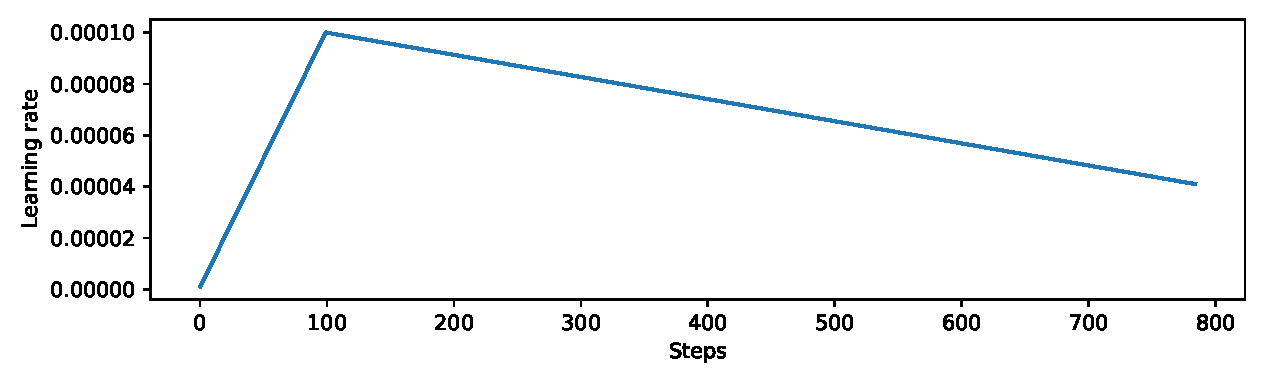
\includegraphics[width=0.47\textwidth]{../images/warmup_linear_schedule.pdf}
    \caption{Learning rate schedule}
    \label{fig:learning-rate-schedule}
\end{figure}

Figure~\ref{fig:loss} shows the loss function value over the fine-tuning process. We do not know why, but loss function shows a greater decrease at the end of each epoch.

\begin{figure}[ht]
    \centering
    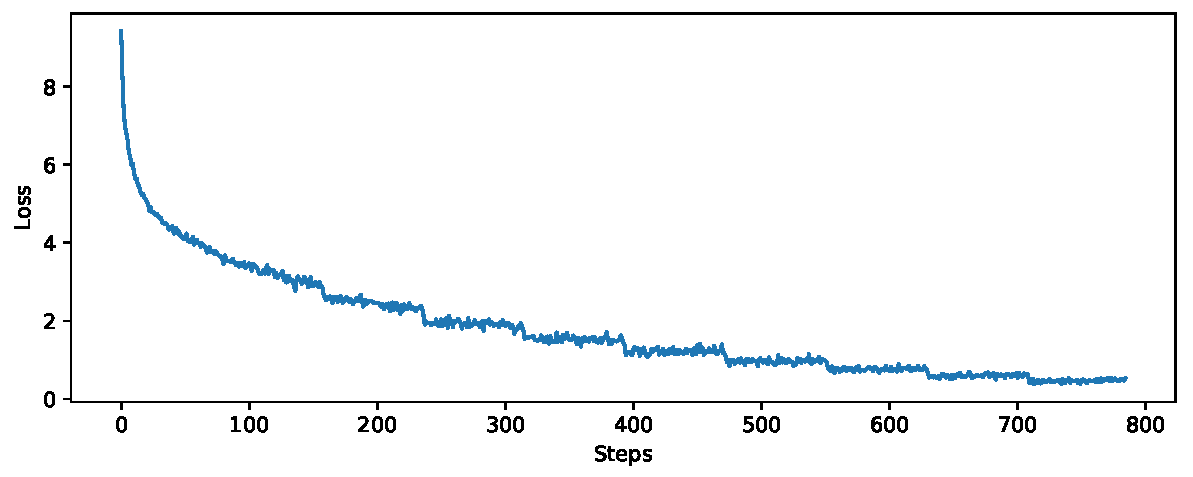
\includegraphics[width=0.47\textwidth]{../images/loss_function.pdf}
    \caption{Loss function}
    \label{fig:loss}
\end{figure}

Some hyperparameters configuration shows bad results in the loss function. For example:

\begin{itemize}
    \item learning rates greater than \num{1e-4} did not make the model converge;
    \item the use of a warm-up period allowed the model to converge in less epochs;
    \item a high number of epochs almost causes an overfitting of the model;
\end{itemize}

The last changed hyperparameter was the number of hypothesis explored in each branch of the beam search. A number greater than \num{3} resulted in more words being out of context in the generated reply email.


\section{Results}

The evaluation of the model was



https://huggingface.co/blog/how-to-generate



\bibliographystyle{aaai}
\bibliography{references}

\end{document}